%%% Template originaly created by Karol Kozioł (mail@karol-koziol.net) and modified for ShareLaTeX use

\documentclass[a4paper,11pt]{article}

\usepackage[T1]{fontenc}
\usepackage[utf8]{inputenc}
\usepackage{graphicx}
\usepackage{xcolor}

\renewcommand\familydefault{\sfdefault}
\usepackage{tgheros}

\usepackage{amsmath,amssymb,amsthm,textcomp}
\usepackage{enumerate}
\usepackage{multicol}
\usepackage{tikz}

\usepackage{geometry}
\geometry{left=25mm,right=25mm,%
bindingoffset=0mm, top=20mm,bottom=20mm}

\usepackage[export]{adjustbox}
\usepackage{subcaption}
\usepackage{float}

\usepackage{amsmath}
\usepackage{amssymb}
\usepackage{amsthm}

\usepackage{geometry}
\geometry{left=25mm,right=25mm,%
bindingoffset=0mm, top=20mm,bottom=20mm}


\linespread{1.3}

\newcommand{\linia}{\rule{\linewidth}{0.5pt}}

% custom theorems if needed
\newtheoremstyle{mytheor}
    {1ex}{1ex}{\normalfont}{0pt}{\scshape}{.}{1ex}
    {{\thmname{#1 }}{\thmnumber{#2}}{\thmnote{ (#3)}}}

\theoremstyle{mytheor}
\newtheorem{defi}{Definition}

% my own titles
\makeatletter
\renewcommand{\maketitle}{
\begin{center}
\vspace{2ex}
{\huge \textsc{\@title}}
\vspace{1ex}
\\
\linia\\
\@author \hfill \@date
\vspace{4ex}
\end{center}
}
\makeatother
%%%

% custom footers and headers
\usepackage{fancyhdr}
\pagestyle{fancy}
\lhead{}
\chead{}
\rhead{}
\cfoot{}
\rfoot{Page \thepage}
\renewcommand{\headrulewidth}{0pt}
\renewcommand{\footrulewidth}{0pt}
%

%%%----------%%%----------%%%----------%%%----------%%%

\begin{document}

\title{Geometria obliczeniowa - Ćwiczenia}

\author{Adrian Mucha 236526, Politechnika Wrocławska WPPT}

\date{25.05.2020}

\maketitle

\section*{Zadanie 25}
Niech $S = \{C_i: (x_i, y_i), i\in[n]\}$ będzie zbiorem $n$ jednostkowych okręgów na płaszczyźnie opisanych wzorem $(x - x_i)^2 + (y - y_i)^2 = 1$ (okręgi mogą się przecinać). Chcemy obliczyć otoczkę wypukłą. Pokażemy, że brzeg otoczki wypukłej składa się z odcinków i kawałków okręgów z $S$, oraz że każdy okrąg może wystąpić co najwyżej raz na brzegu otoczki wypukłej.

\subsection*{Notacja}
\begin{itemize}
    \item $CH(S)$ - otoczka wypukła obejmująca okręgi $S$
    \item $\overline{CH}(S)$ - otoczka wypukła powstała ze środków okręgów
    \item $l(C_i, C_j)$ - odcinek łączący środki $C_i$ oraz $C_j$
\end{itemize}

\subsection*{Rozwiązanie}
Dowód polega na iteracyjnej konstrukcji otoczki wypukłej przy dodawaniu kolejnych okręgów

Rozważmy przypadek podstawowy, dla $n = 1$. Wtedy otoczką wypukłą zbioru jest cały okrąg, w którym brzeg otoczki składa się w całości z okręgu $C_1$ oraz nie posiada odcinków. Otoczka musi w całości przylegać do okręgu, gdyż w przeciwnym wypadku nie byłaby najmniejszą otoczką zawierającą okrąg.

Kolejno dla $n = 2$, w którym brzegi otoczki będą składać się z dwóch stycznych równoległych oraz dwóch półokręgów. Ten przykład jest szczególny i nie spełnia warunku pojedynczego wystąpienia na brzegu otoczki. Jeżeli kolejny okrąg $C_3$ umieścimy pomiędzy $C_1, C_2$ na $l(C_1, C_2)$ to będzie się stykał w dwóch miejscach.

Dodanie $n + 1$-szego okręgu rozbijemy na kilka przypadków. Niech $S_n = \{C_1,\ldots,C_{n}\}$, oraz $S_{n+1} = S_n \cup C_{n+1}$.
\begin{enumerate}
    \item Środek okręgu $C_{n+1}$ znajduje się wewnątrz otoczki wypukłej tworzonej przez środki okręgów $\overline{CH}(S_n)$ (okrąg w całości znajduje się wewnątrz $CH(S_n)$) - otoczka się nie zmienia, nadal jest poprawna. Do tego przypadku również wliczamy okręgi posiadające ten sam środek.
    \item Środek okręgu $C_{n+1}$ znajduje się na brzegu otoczki $\overline{CH}(S_n)$ pomiędzy $C_i$ oraz $C_j$ czyli na prostej $l(C_i, C_j)$. Wówczas okrąg $C_{n+1}$ jest styczny do otoczki $CH(S)$ tylko w jednym punkcie (poza $n = 2$, który był rozważany osobno). Jest to specyficzny przypadek, który zostanie rozwinięty w kolejnym punkcie. 
    \item Okrąg $C_{n+1}$ znajduje się poza otoczką tworzoną przez $CH(S_n)$ - z nowego okręgu wyprowadza się dwie styczne tak, aby były również styczne do otoczki $CH(S_n)$ i nie przecinały się ze sobą jak i innymi prostymi; utworzą one nowe brzegi otoczki. Użycie innych krzywych mogłoby złamać wymagania otoczki wypukłej. Dodatkowo część półkola od punktów styku stycznych jest również dołączana jako brzeg otoczki. Zasada, że okrąg może wystąpić tylko raz na brzegu otoczki nie zostaje złamana. Do nowej (powiększonej) otoczki dodane zostały dwie proste i część okręgu co podtrzymuje warunki postawione na początku zadania.
\end{enumerate}

\begin{figure}
    \centering
    
    \begin{subfigure}{0.4\textwidth}
        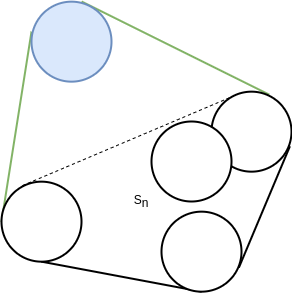
\includegraphics[width=1.0\linewidth]{png/go1.png}
        \caption{}
    \end{subfigure}

    \begin{subfigure}{0.4\textwidth}
        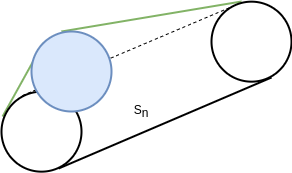
\includegraphics[width=1.0\linewidth]{png/go2.png}
        \caption{}
    \end{subfigure}

    \begin{subfigure}{0.4\textwidth}
        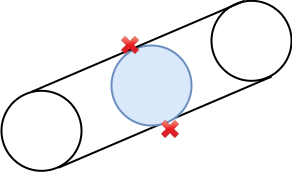
\includegraphics[width=1.0\linewidth]{png/go3.png}
        \caption{}
    \end{subfigure}
\end{figure}

\end{document}